\documentclass[10pt,twocolumn,letterpaper]{article}

\usepackage{cvpr}
\usepackage{times}
\usepackage{epsfig}
\usepackage{graphicx}
\usepackage{amsmath}
\usepackage{amssymb}

% Include other packages here, before hyperref.

% If you comment hyperref and then uncomment it, you should delete
% egpaper.aux before re-running latex.  (Or just hit 'q' on the first latex
% run, let it finish, and you should be clear).
\usepackage[breaklinks=true,bookmarks=false,colorlinks=true]{hyperref}

\cvprfinalcopy % *** Uncomment this line for the final submission

\def\cvprPaperID{****} % *** Enter the CVPR Paper ID here
\def\httilde{\mbox{\tt\raisebox{-.5ex}{\symbol{126}}}}

% Pages are numbered in submission mode, and unnumbered in camera-ready
%\ifcvprfinal\pagestyle{empty}\fi
\setcounter{page}{4321}
\begin{document}

%%%%%%%%% TITLE
\title{CNN-based analysis of organoid growth}

\author{Shan Zhou \\
Facebook \\
\\
{\tt\small shanzhou@stanford.edu}
% For a paper whose authors are all at the same institution,
% omit the following lines up until the closing ``}''.
% Additional authors and addresses can be added with ``\and'',
% just like the second author.
% To save space, use either the email address or home page, not both
\and
Timothy Daley \\
Stanford University \\
Departments of Statistics and Bioengineering \\
{\tt\small tdaley@stanford.edu}
}

\maketitle
%\thispagestyle{empty}

%%%%%%%%% ABSTRACT
\begin{abstract}
   High-throughput analysis of imaging data is critical for analysing large data typical of modern biological investigations.  Here we investigate a convolutional neural network-based approach to analyse the growth of organoids based off of imaging data.  
\end{abstract}

%%%%%%%%% BODY TEXT
\section{Introduction}

Predicting tumor growth rate is a first step in determining treatment options for cancer patients.  Fast growing tumors necessarily require more aggressive treatment.  It would be beneficial if patients could avoid aggressive treatments when possible.  

Alexandra Sockell of the Fordyce and Curtis labs in the Bioengineering and Genetics departments, respectively, of Stanford University has developed a microfluidic device to isolate single cells of a tumor and allow them to grow into organoids  within the microwell.  Organoids are three dimensional stem cell-like cultures that organize into a "mini-organ"~\cite{rios2018imaging}, and can be used to study cancer in a more natural environment than traditional cell lines~\cite{drost2018organoids}.
The objective of her research is to study the mechanisms of tumor growth by subjecting a large number of  individual cells to a wide range of treatments and conditions and track their condition by imaging.  She has taken 14 days of imaging over 8 conditions.    For each day, there are approximate 38,000 well images across all conditions.  The number of cells per well is approximately Poisson, with most of the wells not containing any cells, 25\% have one cell, and smaller portion have more than 1.  We believe that the large number of images should provide a sufficient amount of data and information content to apply deep convolution neural network approach.  Our hypothesis is that the state of the cells in the early days should be related to their final state.  Therefore our objective to determine whether the early stages of the organoid can predict the growth rate and final state of the organoid.    


Previous approaches for high-throughput analysis of organoid imaging data did not look at single-cell microwell level data.  Instead they typically relied upon a large number of cells to quantify cell proliferation or death \cite{jabs2017screening},  used cell counting assays to calculate growth \cite{sebrell2018live}, or used single cell tracking to calculate cell motility \cite{geum2016epidermal}.  To our knowledge, no deep learning approaches have been proposed to analyse organoid imaging data, despite the large success in deep learning to analysing imaging data across a broad spectrum of applications.  We have found successful CNN approaches in related biological analysis such as high content screening \cite{simm2018repurposing}.  

The purpose of this project is to provide a proof of principle for CNN-based high-throughput analysis of organoid imaging data.  

\begin{figure}[b!]
\begin{center}
 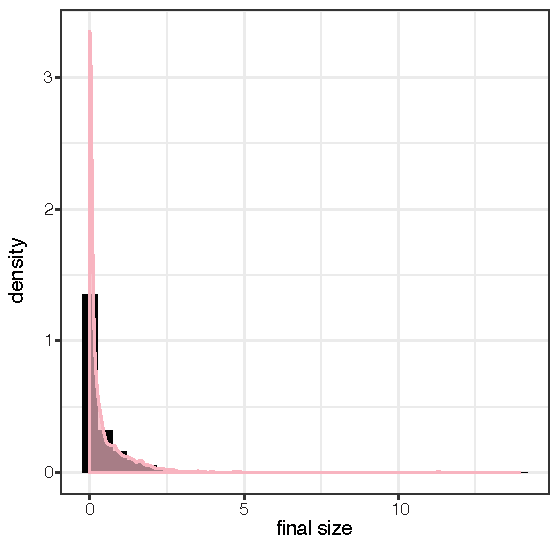
\includegraphics[width=0.8\linewidth]{figures/final_day_hyst2_area_density.pdf}
\end{center}
   \caption{Distribution of normalized final sizes.  There is a large peak at zero corresponding to empty wells or cells that died.}
\label{final_size_dist}
\end{figure}

\section{Data}

%\begin{figure*}[t!]
%\begin{center}
 %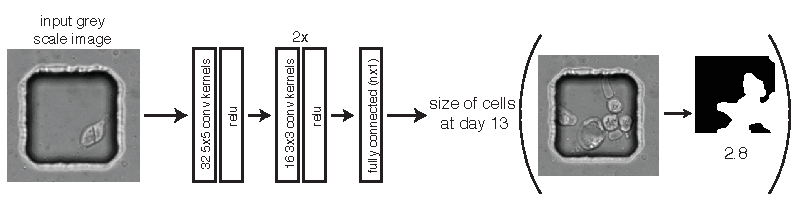
\includegraphics[width=0.8\linewidth]{figures/networkExampleImage.pdf}
%\end{center}
%   \caption{Example workflow of our algorithm.  The input is a 193$\times$193 greyscale image of the cell at day one.  We pass this through a convolutional neural network to predict the final size, normalized to have variance equal to 1.}
%\label{workflow}
%\end{figure*}

The data is composed of 193$\times$193 greyscale images of 4800 microwells for each of 6 wells, imaged across 14 days.  So we have $6 \cdot 4800$ = 28,800 wells with 14 images per well.  The images were obtained via computational stitching~\cite{preibisch2009globally} of multiple larger images of well.  A small number of images appear distorted.  We filtered the images by the estimated area of their interior, computed by the hyst2 function in openCV~\cite{opencv_library}, to try to reduce such artifacts.  If the estimated area was larger than possible for any of the 14 days, then we removed all images of that well from the data.  After filtering we kept 8,763 microwells.  Example images are shown in figure {\color{red} (reference needed)}.

We tried single day image, but day 1 iamge does not work weel. We also tried stacking 2 days or 3 days images for input, the results looks better.

We normalize the input images and size labels by using the training data mean and standard deviation.

We added data augmentation by random cropping with different size and horizonal flipping.

 \section{Methods}
 
 To start we approached the regression problem straightforward.  We found difficulties with overfitting using only day 1 on the images from a single well.  We therefore decided to first focus on the classification problem, to predict from the early days whether the final day is empty or not, using whether the computed hyst2 area is zero or not as zero and one, respectively.   As a proof of principle, we attempted to overtrain a deep convolutional neural network consisting of three convolutional layers, with kernel sizes of 2, 3, and 3, respectively, and channels of 64, 32, 16, respectively.  Each convolutional layers was followed by a batch normalization layer, a ReLU layer, and then a max pooling layer with a kernel size of 2.  The convolutional layer were followed by a square fully connected layer, followed by a ReLU layer, a fully connected layer with output size of one, and finally a sigmoid for output.  We applied this network to all images from a single well, and attempted overfitting on day 1.

 After initial models, we generate two models. The first model is a classification CNN model to find out whether the final day wells has cell or not. We built a five convolutional layer with max pooling and one fully connected layer model with dropout. We compute cross-entropy for loss and use Adam for the optimizer. The model is overfitting for 4000 training images. But when the training set increase to 6000, the validation accuracy incresed to around 0.8. However adding more images to 10000 does not makes the model overffiting again. We then tried adding more regulization like more max pooling and dropout. We also added data augmentation to random crop and rotate the images. We add learning rate decay in the optimizer every 5 steps by 0.1. We also use pretrained ResNet18 mode, the validation accuracy did not increase.

 After finding out which wells has cells by classification model, we predict their final cell sizes by CNN regression model. We used the pretrain ResNet18 model,Adam optimizer and mean square error as loss. 


{\small
\bibliographystyle{ieee}
\bibliography{bib}
}

\end{document}
